% Sezione aggiuntiva: Diagrammi UML di base
\section{Diagrammi UML per OOP Java}
\label{sec:uml_base}

\subsection{Introduzione a UML}

\begin{definizione}
\textbf{UML} (Unified Modeling Language) è un linguaggio di modellazione grafica standardizzato per visualizzare, specificare, costruire e documentare software object-oriented.
\end{definizione}

UML comprende 14 tipi di diagrammi, divisi in:
\begin{itemize}
    \item \textbf{Diagrammi strutturali}: Class diagram, Object diagram, Component diagram, Deployment diagram
    \item \textbf{Diagrammi comportamentali}: Use case diagram, Activity diagram, State machine diagram, Sequence diagram
\end{itemize}

Per Java OOP, i più rilevanti sono i \textbf{Class Diagram}.

\subsection{Class Diagram: Elementi Base}

\subsubsection{Rappresentazione di una classe}

\begin{figure}[H]
\centering
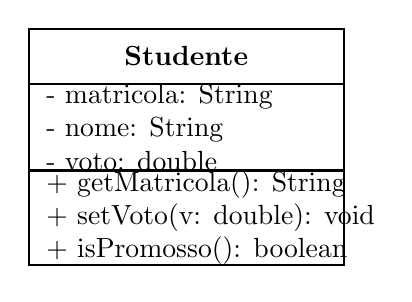
\begin{tikzpicture}
    % Classe completa
    \draw[thick] (0,0) rectangle (4,3);
    \draw[thick] (0,2.3) -- (4,2.3);  % Separatore nome/attributi
    \draw[thick] (0,1.2) -- (4,1.2);  % Separatore attributi/metodi

    % Nome classe
    \node at (2,2.65) {\textbf{Studente}};

    % Attributi
    \node[align=left] at (0.1,1.75) [anchor=west] {
        - matricola: String \\
        - nome: String \\
        - voto: double
    };

    % Metodi
    \node[align=left] at (0.1,0.6) [anchor=west] {
        + getMatricola(): String \\
        + setVoto(v: double): void \\
        + isPromosso(): boolean
    };
\end{tikzpicture}
\caption{Struttura classe UML: Nome, Attributi, Metodi}
\end{figure}

\textbf{Convenzioni}:
\begin{itemize}
    \item \textbf{Nome classe}: Centrato, grassetto, PascalCase
    \item \textbf{Attributi}: Formato \texttt{visibilità nome: tipo}
    \item \textbf{Metodi}: Formato \texttt{visibilità nome(parametri): tipoRitorno}
    \item \textbf{Visibilità}:
    \begin{itemize}
        \item \texttt{+} = public
        \item \texttt{-} = private
        \item \texttt{\#} = protected
        \item \texttt{\textasciitilde} = package (default)
    \end{itemize}
\end{itemize}

\subsubsection{Attributi e metodi static}

Gli elementi static si sottolineano:

\begin{figure}[H]
\centering
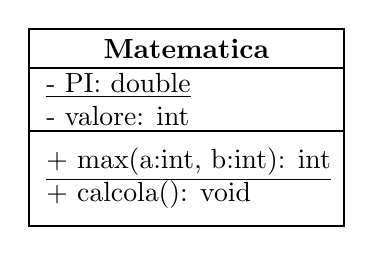
\begin{tikzpicture}
    \draw[thick] (0,0) rectangle (4,2.5);
    \draw[thick] (0,2) -- (4,2);
    \draw[thick] (0,1.2) -- (4,1.2);

    \node at (2,2.25) {\textbf{Matematica}};

    \node[align=left] at (0.1,1.6) [anchor=west] {
        \underline{- PI: double} \\
        - valore: int
    };

    \node[align=left] at (0.1,0.6) [anchor=west] {
        \underline{+ max(a:int, b:int): int} \\
        + calcola(): void
    };
\end{tikzpicture}
\caption{Sottolineatura per membri static}
\end{figure}

\subsubsection{Classi astratte e interfacce}

\begin{figure}[H]
\centering
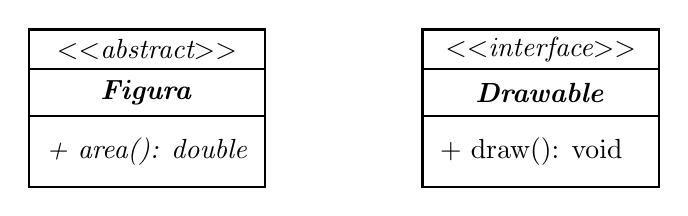
\begin{tikzpicture}
    % Classe astratta
    \draw[thick] (0,0) rectangle (3,2);
    \draw[thick] (0,1.5) -- (3,1.5);
    \draw[thick] (0,0.9) -- (3,0.9);

    \node at (1.5,1.75) {\textit{\textless\textless abstract\textgreater\textgreater}};
    \node at (1.5,1.2) {\textit{\textbf{Figura}}};

    \node[align=left] at (0.1,0.45) [anchor=west] {
        \textit{+ area(): double}
    };

    % Interfaccia
    \draw[thick] (5,0) rectangle (8,2);
    \draw[thick] (5,1.5) -- (8,1.5);
    \draw[thick] (5,0.9) -- (8,0.9);

    \node at (6.5,1.75) {\textit{\textless\textless interface\textgreater\textgreater}};
    \node at (6.5,1.2) {\textit{\textbf{Drawable}}};

    \node[align=left] at (5.1,0.45) [anchor=west] {
        + draw(): void
    };
\end{tikzpicture}
\caption{Classe astratta vs Interfaccia (nome in corsivo)}
\end{figure}

\subsection{Relazioni tra Classi}

\subsubsection{1. Ereditarietà (Generalization)}

Freccia con punta triangolare vuota dalla sottoclasse alla superclasse.

\begin{figure}[H]
\centering
\begin{tikzpicture}[
    class/.style={rectangle, draw, rounded corners, minimum width=3.5cm, minimum height=1cm, fill=blue!5},
    inherit/.style={-{Triangle[open, length=3mm, width=4mm]}, thick}
]
    % Superclasse
    \node[class] (veicolo) at (0,3) {
        \textbf{Veicolo} \\
        \small - velocità: int \\
        \small + muovi(): void
    };

    % Sottoclassi
    \node[class] (auto) at (-3,0) {
        \textbf{Auto} \\
        \small - numPorte: int \\
        \small + apriPorta(): void
    };

    \node[class] (moto) at (3,0) {
        \textbf{Moto} \\
        \small - cilindrata: int \\
        \small + impenna(): void
    };

    % Frecce ereditarietà
    \draw[inherit] (auto) -- (veicolo);
    \draw[inherit] (moto) -- (veicolo);
\end{tikzpicture}
\caption{Ereditarietà: Auto e Moto estendono Veicolo}
\end{figure}

\textbf{Codice Java corrispondente}:
\begin{lstlisting}[language=Java]
public class Veicolo {
    private int velocità;
    public void muovi() { /* ... */ }
}

public class Auto extends Veicolo {
    private int numPorte;
    public void apriPorta() { /* ... */ }
}

public class Moto extends Veicolo {
    private int cilindrata;
    public void impenna() { /* ... */ }
}
\end{lstlisting}

\subsubsection{2. Implementazione di Interfaccia (Realization)}

Freccia tratteggiata con punta triangolare vuota dalla classe all'interfaccia.

\begin{figure}[H]
\centering
\begin{tikzpicture}[
    class/.style={rectangle, draw, rounded corners, minimum width=3cm, minimum height=0.8cm, fill=blue!5},
    interface/.style={rectangle, draw, rounded corners, minimum width=3cm, minimum height=0.8cm, fill=green!5},
    realize/.style={-{Triangle[open, length=3mm, width=4mm]}, thick, dashed}
]
    \node[interface] (comp) at (0,2.5) {
        \textit{\textless\textless interface\textgreater\textgreater} \\
        \textbf{Comparable}
    };

    \node[class] (studente) at (0,0) {
        \textbf{Studente} \\
        \small + compareTo(s): int
    };

    \draw[realize] (studente) -- (comp);
\end{tikzpicture}
\caption{Implementazione: Studente implements Comparable}
\end{figure}

\subsubsection{3. Associazione}

Linea continua tra classi che collaborano. Può avere:
\begin{itemize}
    \item \textbf{Molteplicità}: Quanti oggetti sono coinvolti (0..1, 1, *, 0..*, 1..*)
    \item \textbf{Ruoli}: Nomi alle estremità
    \item \textbf{Navigabilità}: Frecce indicano direzione accesso
\end{itemize}

\begin{figure}[H]
\centering
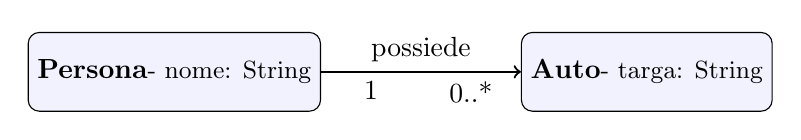
\begin{tikzpicture}[
    class/.style={rectangle, draw, rounded corners, minimum width=3cm, minimum height=1cm, fill=blue!5}
]
    \node[class] (persona) at (0,0) {
        \textbf{Persona} \\
        \small - nome: String
    };

    \node[class] (auto) at (6,0) {
        \textbf{Auto} \\
        \small - targa: String
    };

    \draw[->, thick] (persona) -- node[above] {possiede} node[below, near start] {1} node[below, near end] {0..*} (auto);
\end{tikzpicture}
\caption{Associazione: Persona possiede 0 o più Auto}
\end{figure}

\textbf{Molteplicità comune}:
\begin{itemize}
    \item \texttt{1}: Esattamente uno
    \item \texttt{0..1}: Zero o uno (opzionale)
    \item \texttt{*} o \texttt{0..*}: Zero o più
    \item \texttt{1..*}: Uno o più
    \item \texttt{n..m}: Da n a m (es: 2..5)
\end{itemize}

\subsubsection{4. Aggregazione}

Relazione "ha-un" debole (il contenuto può esistere indipendentemente). Rombo vuoto.

\begin{figure}[H]
\centering
\begin{tikzpicture}[
    class/.style={rectangle, draw, rounded corners, minimum width=3cm, minimum height=1cm, fill=blue!5}
]
    \node[class] (dipartimento) at (0,0) {
        \textbf{Dipartimento} \\
        \small - nome: String
    };

    \node[class] (professore) at (6,0) {
        \textbf{Professore} \\
        \small - nome: String
    };

    \draw[-{Diamond[open, length=3mm, width=3mm]}, thick] (professore) -- node[above] {lavora in} node[below, near start] {*} node[below, near end] {1} (dipartimento);
\end{tikzpicture}
\caption{Aggregazione: Dipartimento ha Professori (che possono esistere indipendentemente)}
\end{figure}

\subsubsection{5. Composizione}

Relazione "ha-un" forte (il contenuto non può esistere senza il contenitore). Rombo pieno.

\begin{figure}[H]
\centering
\begin{tikzpicture}[
    class/.style={rectangle, draw, rounded corners, minimum width=3cm, minimum height=1cm, fill=blue!5}
]
    \node[class] (casa) at (0,0) {
        \textbf{Casa} \\
        \small - indirizzo: String
    };

    \node[class] (stanza) at (6,0) {
        \textbf{Stanza} \\
        \small - dimensione: double
    };

    \draw[-{Diamond[fill, length=3mm, width=3mm]}, thick] (stanza) -- node[above] {è parte di} node[below, near start] {1..*} node[below, near end] {1} (casa);
\end{tikzpicture}
\caption{Composizione: Casa composta da Stanze (che non esistono senza Casa)}
\end{figure}

\textbf{Codice Java}:
\begin{lstlisting}[language=Java]
public class Casa {
    private List<Stanza> stanze;  // Composizione

    public Casa() {
        stanze = new ArrayList<>();
        stanze.add(new Stanza("Cucina"));    // Stanze create con Casa
        stanze.add(new Stanza("Soggiorno"));
    }
}
\end{lstlisting}

\subsubsection{6. Dipendenza}

Relazione temporanea (una classe usa l'altra come parametro). Freccia tratteggiata.

\begin{figure}[H]
\centering
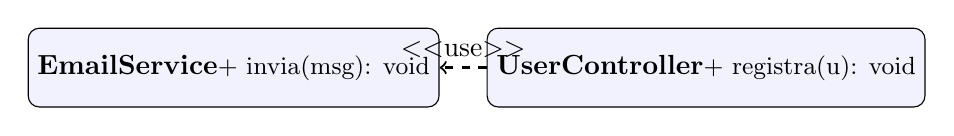
\begin{tikzpicture}[
    class/.style={rectangle, draw, rounded corners, minimum width=3cm, minimum height=1cm, fill=blue!5}
]
    \node[class] (servizio) at (0,0) {
        \textbf{EmailService} \\
        \small + invia(msg): void
    };

    \node[class] (controller) at (6,0) {
        \textbf{UserController} \\
        \small + registra(u): void
    };

    \draw[->, thick, dashed] (controller) -- node[above] {\textless\textless use\textgreater\textgreater} (servizio);
\end{tikzpicture}
\caption{Dipendenza: UserController usa EmailService temporaneamente}
\end{figure}

\subsection{Esempio Completo: Sistema Biblioteca}

\begin{figure}[H]
\centering
\begin{tikzpicture}[
    scale=0.8,
    every node/.style={scale=0.8},
    class/.style={rectangle, draw, rounded corners, minimum width=3cm, minimum height=1.2cm, fill=blue!5},
    interface/.style={rectangle, draw, rounded corners, minimum width=3cm, minimum height=0.9cm, fill=green!5},
    inherit/.style={-{Triangle[open, length=2.5mm, width=3.5mm]}, thick},
    realize/.style={-{Triangle[open, length=2.5mm, width=3.5mm]}, thick, dashed},
    assoc/.style={->, thick},
    compos/.style={-{Diamond[fill, length=2.5mm, width=2.5mm]}, thick}
]
    % Interfaccia
    \node[interface] (prestabile) at (0,5) {
        \textit{\textless\textless interface\textgreater\textgreater} \\
        \textbf{Prestabile}
    };

    % Classe astratta
    \node[class] (materiale) at (0,3) {
        \textit{\textbf{MaterialeBibliotecario}} \\
        \small - codice: String \\
        \small + getCodice(): String
    };

    % Classi concrete
    \node[class] (libro) at (-3,0) {
        \textbf{Libro} \\
        \small - isbn: String \\
        \small + prestito(): void
    };

    \node[class] (rivista) at (3,0) {
        \textbf{Rivista} \\
        \small - numero: int \\
        \small + prestito(): void
    };

    % Biblioteca
    \node[class] (biblioteca) at (8,1.5) {
        \textbf{Biblioteca} \\
        \small - nome: String \\
        \small + aggiungi(m): void
    };

    % Utente
    \node[class] (utente) at (8,-1.5) {
        \textbf{Utente} \\
        \small - nome: String \\
        \small + presta(m): void
    };

    % Relazioni
    \draw[realize] (materiale) -- (prestabile);
    \draw[inherit] (libro) -- (materiale);
    \draw[inherit] (rivista) -- (materiale);
    \draw[compos] (materiale) -- node[above, sloped] {contiene} node[below, near start] {*} node[below, near end] {1} (biblioteca);
    \draw[assoc] (utente) -- node[above, sloped] {prende in prestito} node[below, near start] {*} node[below, near end] {0..*} (libro);
\end{tikzpicture}
\caption{Diagramma UML completo sistema biblioteca}
\end{figure}

\textbf{Legenda relazioni}:
\begin{itemize}
    \item MaterialeBibliotecario \textit{realizza} Prestabile (interfaccia)
    \item Libro e Rivista \textit{ereditano} da MaterialeBibliotecario
    \item Biblioteca \textit{è composta} da MaterialeBibliotecario
    \item Utente \textit{è associato} a Libro (prestito)
\end{itemize}

\subsection{Tabella Riepilogo Relazioni}

\begin{table}[H]
\centering
\small
\begin{tabular}{lll}
\toprule
\textbf{Relazione} & \textbf{Simbolo UML} & \textbf{Codice Java} \\
\midrule
Ereditarietà & Freccia triangolo vuoto & \texttt{extends} \\
Implementazione & Freccia tratteggiata triangolo vuoto & \texttt{implements} \\
Associazione & Linea continua (opz. freccia) & Attributo di tipo classe \\
Aggregazione & Rombo vuoto & Attributo (indipendente) \\
Composizione & Rombo pieno & Attributo (dipendente) \\
Dipendenza & Freccia tratteggiata & Parametro metodo \\
\bottomrule
\end{tabular}
\caption{Mappatura UML - Java}
\end{table}

\subsection{Tool per UML}

\textbf{Software diagrammi UML}:
\begin{itemize}
    \item \textbf{PlantUML}: Diagrammi da testo: \url{https://plantuml.com/}
    \item \textbf{draw.io}: Editor online gratuito: \url{https://draw.io/}
    \item \textbf{Lucidchart}: Collaborativo online: \url{https://www.lucidchart.com/}
    \item \textbf{Visual Paradigm}: Professionale (trial gratuito)
    \item \textbf{StarUML}: Open source: \url{http://staruml.io/}
    \item \textbf{IntelliJ IDEA Ultimate}: Plugin UML integrato
    \item \textbf{Eclipse Papyrus}: Plugin UML per Eclipse
\end{itemize}

\textbf{Esempio PlantUML}:
\begin{lstlisting}[language=Java]
@startuml
class Veicolo {
  - velocità: int
  + muovi(): void
}

class Auto {
  - numPorte: int
}

class Moto {
  - cilindrata: int
}

Veicolo <|-- Auto
Veicolo <|-- Moto
@enduml
\end{lstlisting}

\subsection{Best Practices UML}

\begin{enumerate}
    \item \textbf{Semplicità}: Mostrare solo dettagli rilevanti
    \item \textbf{Chiarezza}: Nomi descrittivi, layout ordinato
    \item \textbf{Coerenza}: Usare convenzioni standard UML 2.x
    \item \textbf{Livello di dettaglio appropriato}:
    \begin{itemize}
        \item Conceptual: Solo nomi classi e relazioni principali
        \item Specification: Include firme metodi pubblici
        \item Implementation: Tutti attributi e metodi
    \end{itemize}
    \item \textbf{Documentare assunzioni}: Note per chiarire scelte design
\end{enumerate}

\begin{nota}
UML è uno strumento di comunicazione, non un fine. Usare il livello di dettaglio necessario per il contesto (progettazione, documentazione, presentazione).
\end{nota}

\subsection{Esercizi UML}

\begin{esercizio}[UML.1]
Disegnare diagramma classi UML per sistema gestione studenti con classi: Studente, Corso, Professore. Includere relazioni appropriate.
\end{esercizio}

\begin{esercizio}[UML.2]
Dato il seguente codice, creare diagramma UML completo:
\begin{lstlisting}[language=Java]
public abstract class Animal {
    protected String nome;
    public abstract void verso();
}

public class Cane extends Animal {
    public void verso() { System.out.println("Bau!"); }
}

public interface Addestrabile {
    void addestra(String comando);
}
\end{lstlisting}
\end{esercizio}

\begin{esercizio}[UML.3]
Identificare e spiegare gli errori in un diagramma UML fornito (da creare dal docente con errori intenzionali: molteplicità sbagliata, frecce invertite, etc.).
\end{esercizio}
